% !TEX program = tectonic
% Deck AUTONOME « Les autres dépôts & la construction de portefeuille » (Chambre).
% Même format que 00_recuperation_donnees/SLIDES_DONNEES.tex (thème Madrid, couleurs, macros).
% But : remettre les chiffres au clair (anti-confusion) + développer complètement
% « comment ça change la construction de portefeuille » (notebook 10 / FICHE_10).
% Chiffres : ANALYSE_FILING_TYPES_HOUSE.md · V1_House.ipynb · 10_Stock_Divulgations_MathSpec.ipynb.
% Millésime unique = UNION (35 377 dépôts). Additif : ne modifie ni V2 ni le notebook 10.
\documentclass[11pt,aspectratio=169]{beamer}
\definecolor{helec}{HTML}{3B6EA5}   % couleur maîtresse (Chambre électronique)
\usetheme{Madrid}
\usecolortheme[named=helec]{structure}
\setbeamertemplate{navigation symbols}{}
\setbeamertemplate{blocks}[rounded][shadow=false]
\setbeamerfont{frametitle}{series=\bfseries}
\usepackage[T1]{fontenc}
\usepackage{lmodern}
\usepackage[utf8]{inputenc}
\usepackage[french]{babel}
\usepackage{booktabs}
\usepackage{xcolor}
\usepackage{graphicx}
\usepackage{amssymb}
\usepackage{amsmath}
\usepackage{array}
\usepackage{newunicodechar}
\usepackage{tikz}
\usetikzlibrary{arrows.meta,positioning,calc}
\hypersetup{colorlinks=true, urlcolor=helec, linkcolor=white}

% Caractères Unicode → commandes (fontes T1)
\newunicodechar{→}{\ensuremath{\rightarrow}}
\newunicodechar{—}{\textemdash}
\newunicodechar{–}{\textendash}
\newunicodechar{…}{\ldots}
\newunicodechar{·}{\textperiodcentered}
\newunicodechar{≈}{\ensuremath{\approx}}
\newunicodechar{×}{\ensuremath{\times}}
\newunicodechar{≤}{\ensuremath{\leq}}
\newunicodechar{≥}{\ensuremath{\geq}}
\newunicodechar{−}{\ensuremath{-}}
\newunicodechar{✓}{\checkmark}
\newunicodechar{↔}{\ensuremath{\leftrightarrow}}
\newunicodechar{≠}{\ensuremath{\neq}}
\newunicodechar{⊇}{\ensuremath{\supseteq}}
\newunicodechar{∑}{\ensuremath{\textstyle\sum}}
\newunicodechar{∧}{\ensuremath{\wedge}}
\newunicodechar{œ}{\oe}
\newunicodechar{Œ}{\OE}
\newunicodechar{°}{\textdegree}
\newunicodechar{§}{\S}
\newunicodechar{«}{\og}
\newunicodechar{»}{\fg{}}

% Code couleur (repris de V2)
\definecolor{helec}{HTML}{3B6EA5}   % Chambre électronique / reconstruction
\definecolor{hocr}{HTML}{A9C5E2}
\definecolor{okgreen}{HTML}{2E8B57}
\definecolor{alertred}{HTML}{C0392B}
\definecolor{warnorange}{HTML}{E67E22}
\definecolor{dataC}{RGB}{176,110,14}  % ocre — « données / autres dépôts »
\definecolor{grisC}{RGB}{90,90,90}

\newcommand{\co}[1]{\texttt{#1}}
\tikzset{
  step/.style={rectangle, rounded corners=2pt, draw=#1, line width=0.8pt, fill=#1!8,
               align=center, font=\scriptsize, minimum height=0.72cm},
  bande/.style={rectangle, rounded corners=2pt, draw=#1, line width=0.8pt, fill=#1!8,
                align=center, font=\scriptsize, minimum height=0.62cm},
  arr/.style={-{Latex[length=2mm]}, line width=0.8pt, draw=gray!65},
}

\newcommand{\badge}[2]{\colorbox{#1}{\textcolor{white}{\footnotesize\textbf{#2}}}}
\newcommand{\kpi}[3]{{\large\textbf{\textcolor{#1}{#2}}}~{\footnotesize #3}}
\newcommand{\defl}[1]{{\scriptsize\color{black!55}#1}}

% Carreau chiffre-clé : \tuile{couleur}{gros chiffre}{légende}
\newcommand{\tuile}[3]{%
  \begin{minipage}[t]{0.23\textwidth}\centering
    \colorbox{#1}{\parbox[c][20mm][c]{\dimexpr\linewidth-8pt}{\centering
      {\color{white}\Large\textbf{#2}}\\[0.5mm]{\color{white}\footnotesize #3}}}
  \end{minipage}}

% ── Fil conducteur de la COLLECTE : \pipefigFD{k} ──
% Un seul dessin linéaire à 6 gestes ; seule l'étape k reste allumée (curseur « vous êtes ici »).
% k=0 → tout allumé (vue d'ensemble). Mécanisme d'opacité repris de \pipefig (V2).
\tikzset{pbox/.style n args={2}{rectangle, rounded corners=3pt, draw=#1, fill=#1!10, line width=1pt,
  align=center, font=\scriptsize, text width=2.15cm, minimum height=1.15cm, opacity=#2, text opacity=#2}}
\newcommand{\pipefigFD}[1]{%
  \def\opA{0.16}\def\opB{0.16}\def\opC{0.16}\def\opD{0.16}\def\opE{0.16}\def\opF{0.16}%
  \ifnum#1=0 \def\opA{1}\def\opB{1}\def\opC{1}\def\opD{1}\def\opE{1}\def\opF{1}\fi
  \ifnum#1=1 \def\opA{1}\fi \ifnum#1=2 \def\opB{1}\fi \ifnum#1=3 \def\opC{1}\fi
  \ifnum#1=4 \def\opD{1}\fi \ifnum#1=5 \def\opE{1}\fi \ifnum#1=6 \def\opF{1}\fi
  \begin{tikzpicture}[node distance=3mm, every node/.style={transform shape}]
    \node[pbox={helec}{\opA}] (a) {\textbf{1 · RECENSER}\\{\tiny 35\,377 dépôts}};
    \node[pbox={helec}{\opB}, right=of a] (b) {\textbf{2 · ROUTER}\\{\tiny lisible / scanné}};
    \node[pbox={helec}{\opC}, right=of b] (c) {\textbf{3 · IDENTIFIER}\\{\tiny nom → bioguide}};
    \node[pbox={dataC}{\opD}, right=of c] (d) {\textbf{4 · EXTRAIRE}\\{\tiny regex / OCR}};
    \node[pbox={dataC}{\opE}, right=of d] (e) {\textbf{5 · TABLES}\\{\tiny 18 tables}};
    \node[pbox={okgreen}{\opF}, right=of e] (f) {\textbf{6 · BOUCLE}\\{\tiny Σ = 35\,377 ✓}};
    \draw[arr,opacity=0.35] (a)--(b); \draw[arr,opacity=0.35] (b)--(c); \draw[arr,opacity=0.35] (c)--(d);
    \draw[arr,opacity=0.35] (d)--(e); \draw[arr,opacity=0.35] (e)--(f);
  \end{tikzpicture}}
% Bandeau « vous êtes ici » : le pipeline à taille réduite, en haut d'une frame d'étape.
\newcommand{\pipestrip}[1]{\resizebox{0.98\textwidth}{!}{\pipefigFD{#1}}}

% Encadré CHOIX (un choix méthodologique énoncé en une phrase)
\newcommand{\choixbox}[1]{%
  \colorbox{alertred!8}{\parbox{\dimexpr\linewidth-8pt}{\scriptsize
    \textbf{\textcolor{alertred}{CHOIX}}\; --- #1}}}
% Bandeau RÉPONSE (conclusion d'une partie)
\newcommand{\repband}[1]{%
  \colorbox{okgreen!12}{\parbox{\dimexpr\linewidth-10pt}{\scriptsize
    \textbf{\textcolor{okgreen}{Réponse}}\; --- #1}}}

% Séparateur de partie plein cadre : \partdivider{couleur}{ACTE X}{Grand titre}{sous-titre}
\newcommand{\partdivider}[4]{%
  {\setbeamercolor{background canvas}{bg=#1}
  \begin{frame}[plain]
    \centering\vfill
    {\color{white}\Large\textbf{#2}}\\[3.5mm]
    {\color{white!75}\rule{0.40\textwidth}{1pt}}\\[4.5mm]
    {\color{white}\fontsize{30}{34}\selectfont\textbf{#3}}\\[5.5mm]
    {\color{white!88}\large #4}
    \vfill
  \end{frame}}}

% Pied de page = réplique Madrid ; total = dernière page de contenu (\label{endmain}).
\setbeamertemplate{footline}{%
  \leavevmode%
  \hbox{%
  \begin{beamercolorbox}[wd=.333333\paperwidth,ht=2.25ex,dp=1ex,center]{author in head/foot}%
    \usebeamerfont{author in head/foot}\insertshortauthor~(\insertshortinstitute)%
  \end{beamercolorbox}%
  \begin{beamercolorbox}[wd=.333333\paperwidth,ht=2.25ex,dp=1ex,center]{title in head/foot}%
    \usebeamerfont{title in head/foot}\insertshorttitle%
  \end{beamercolorbox}%
  \begin{beamercolorbox}[wd=.333333\paperwidth,ht=2.25ex,dp=1ex,right]{title in head/foot}%
    \usebeamerfont{title in head/foot}\insertshortdate{}\hspace*{2em}%
    \insertframenumber{} / \pageref{endmain}\hspace*{2ex}%
  \end{beamercolorbox}}%
  \vskip0pt%
}

\title[Les autres dépôts]{Les autres dépôts --- le patrimoine, sa reconstruction,\\ et ce qu'il change au backtest}
\subtitle{Déclarations boursières du Congrès américain · Chambre · 2014--2026}
\author[A.~Lemaire]{Alice Lemaire}
\institute[Ramify]{Document de recherche --- livrable Ramify}
\date{Juillet 2026}

\begin{document}

% ══════════════════════════ TITRE ══════════════════════════
\begin{frame}[plain]
  \titlepage
\end{frame}

% ══════════════════════════ LE FIL ══════════════════════════
\begin{frame}{Le fil --- quatre actes, dans l'ordre}
  \vspace{1mm}
  \begin{columns}[T]
  \column{0.24\textwidth}
    \colorbox{helec!12}{\parbox[t][3.7cm][t]{\dimexpr\linewidth-8pt}{\vspace{0.6mm}
      {\color{helec}\bfseries ACTE 1}\\[1mm]
      \textbf{De la source aux tables}\\[1.2mm]
      {\scriptsize comment on \textbf{récupère} \& extrait la donnée : électronique vs scanné, l'OCR, les 18 tables}}}
  \column{0.24\textwidth}
    \colorbox{dataC!12}{\parbox[t][3.7cm][t]{\dimexpr\linewidth-8pt}{\vspace{0.6mm}
      {\color{dataC}\bfseries ACTE 2}\\[1mm]
      \textbf{Les chiffres au clair}\\[1.2mm]
      {\scriptsize le catalogue des 12 types + les nombres, sans se perdre}}}
  \column{0.24\textwidth}
    \colorbox{helec!12}{\parbox[t][3.7cm][t]{\dimexpr\linewidth-8pt}{\vspace{0.6mm}
      {\color{helec}\bfseries ACTE 3}\\[1mm]
      \textbf{La population : qui a quoi}\\[1.2mm]
      {\scriptsize portefeuille d'entrée, vérifiable, annuels --- 822 reconstruits, 56 prouvés}}}
  \column{0.24\textwidth}
    \colorbox{okgreen!14}{\parbox[t][3.7cm][t]{\dimexpr\linewidth-8pt}{\vspace{0.6mm}
      {\color{okgreen}\bfseries ACTE 4}\\[1mm]
      \textbf{Changer le portefeuille}\\[1.2mm]
      {\scriptsize partir du patrimoine d'entrée --- ce que ça change vraiment}}}
  \end{columns}
  \vspace{3mm}
  {\footnotesize\color{black!60} Périmètre : \textbf{Chambre} uniquement · un seul millésime de comptage (\textbf{union}, 35\,377 dépôts) · chaque chiffre sort d'un notebook exécuté (V1-House, notebook 10).}
\end{frame}

% ════════════════════════════════════════════════════════════
% ════════════════════════════════════════════════════════════
\partdivider{helec}{ACTE 1}{De la source aux tables}{comment on récupère la donnée déclarative --- avant de parler de population ou de backtest}

% ── A0 · le même pipeline que le PTR, sauf un geste ──
\begin{frame}{Le trajet --- le même pipeline que le PTR, sauf un geste}
  \centering\vspace{1mm}
  \pipestrip{0}\\[4mm]
  {\footnotesize les gestes \textbf{1 à 3} (recenser · router · identifier) et le \textbf{mécanisme d'OCR} sont \textbf{identiques au PTR} --- déjà vus. Le seul qui \textbf{change} est le geste \textbf{4 · extraire} : on ne lit pas la même chose \emph{dans} le document.}\\[3mm]
  \choixbox{on ne re-raconte donc pas le pipeline du PTR : on va droit à \textbf{ce qui diffère} --- les \emph{schedules} du formulaire FD.}
\end{frame}

% ── A1 · rappel : recenser / router / identifier = pipeline PTR ──
\begin{frame}{Rappel --- recenser, router, identifier : c'est le pipeline du PTR}
  \centering\vspace{1mm}
  \begin{columns}[c]
  \column{0.53\textwidth}
   \begin{itemize}\footnotesize
    \item[\textbf{1}] \textbf{Recenser} : 13 index annuels → \textbf{35\,377} dépôts (dont 27\,110 « autres »).
    \item[\textbf{2}] \textbf{Router} : le 1\up{er} chiffre du \co{DocID} → \textbf{lisible} (\co{1}-\co{4}) ou \textbf{scanné} (\co{7}-\co{9}).
    \item[\textbf{3}] \textbf{Identifier} : nom imprimé → \co{bioguide} (rattachement 99 \%).
   \end{itemize}
   \vspace{1.5mm}
   \choixbox{rien de neuf ici --- \textbf{c'est le pipeline du PTR}. Une seule nuance : les FD ont une part \textbf{scannée plus lourde} (annuels papier) → plus d'OCR.}
  \column{0.45\textwidth}
   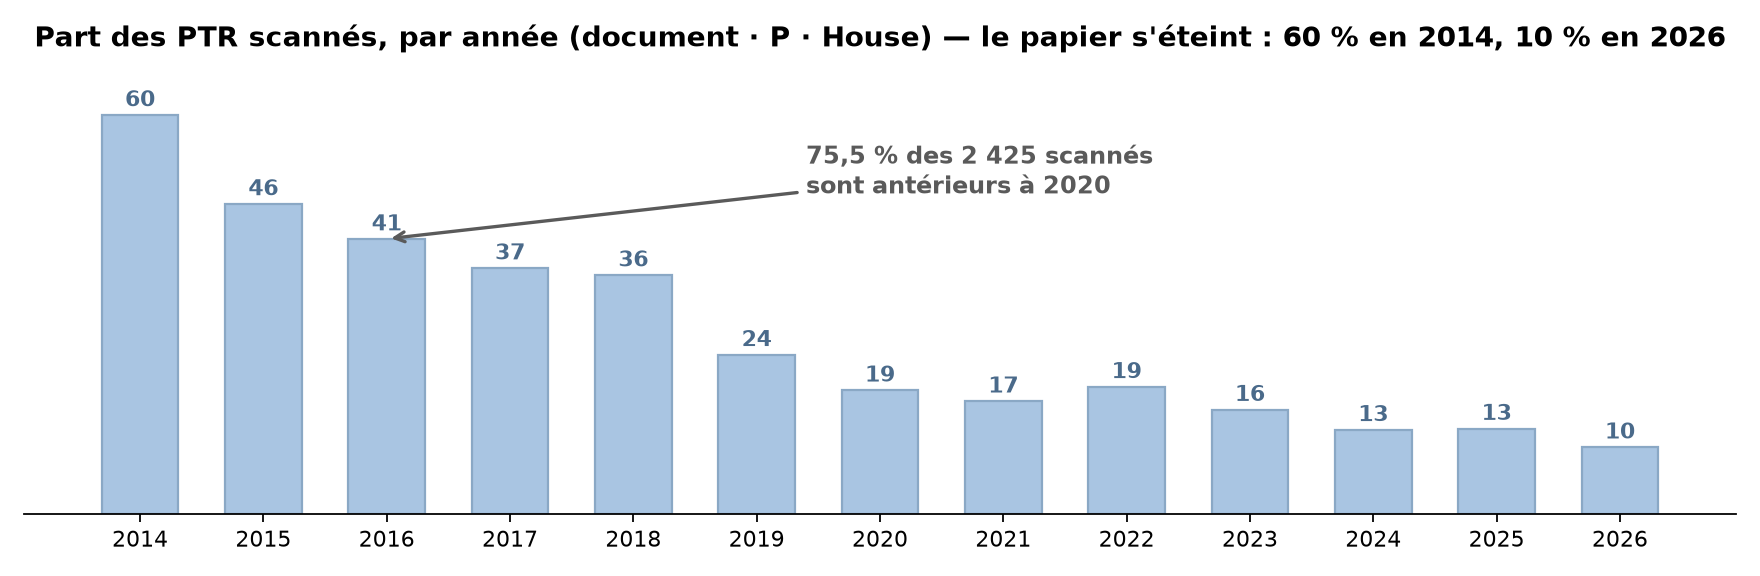
\includegraphics[width=\linewidth,height=0.55\textheight,keepaspectratio]{figs_depots/fig_house_scans_par_annee.png}\\[1mm]
   {\scriptsize\color{black!55} part scannée par année (2014--2019 surtout).}
  \end{columns}
\end{frame}

% ── A2 · la vraie différence : un formulaire, dix sections ──
\begin{frame}{4 · Extraire --- la vraie différence : un formulaire à dix sections}
  \centering\pipestrip{4}\\[3mm]
  \begin{columns}[c]
  \column{0.5\textwidth}
   {\footnotesize le \textbf{PTR} n'a qu'\textbf{une} section --- \co{B} (transactions). Un \textbf{FD} (\co{C}/\co{O}/\co{H}/\co{T}/\co{A}) en a \textbf{dix} :}\\[2mm]
   \begin{tikzpicture}[node distance=1.6mm]
     \node[bande=grisC, text width=5.8cm] (p){\textbf{PTR} : \co{B} seul → transactions};
     \node[bande=dataC, text width=5.8cm, below=of p] (f){\textbf{FD} : \co{A} \co{B} \co{C} \co{D} \co{E} \co{F} \co{G} \co{H} \co{I} \co{J}};
   \end{tikzpicture}\\[2.5mm]
   {\footnotesize on les \textbf{distingue par leurs en-têtes} \co{SCHEDULE A:} … \co{SCHEDULE J:} --- un découpage qui gère deux mises en page (« ScHeDule b: » $\leq$ 2020, « S B: » 2021+).}
  \column{0.48\textwidth}
   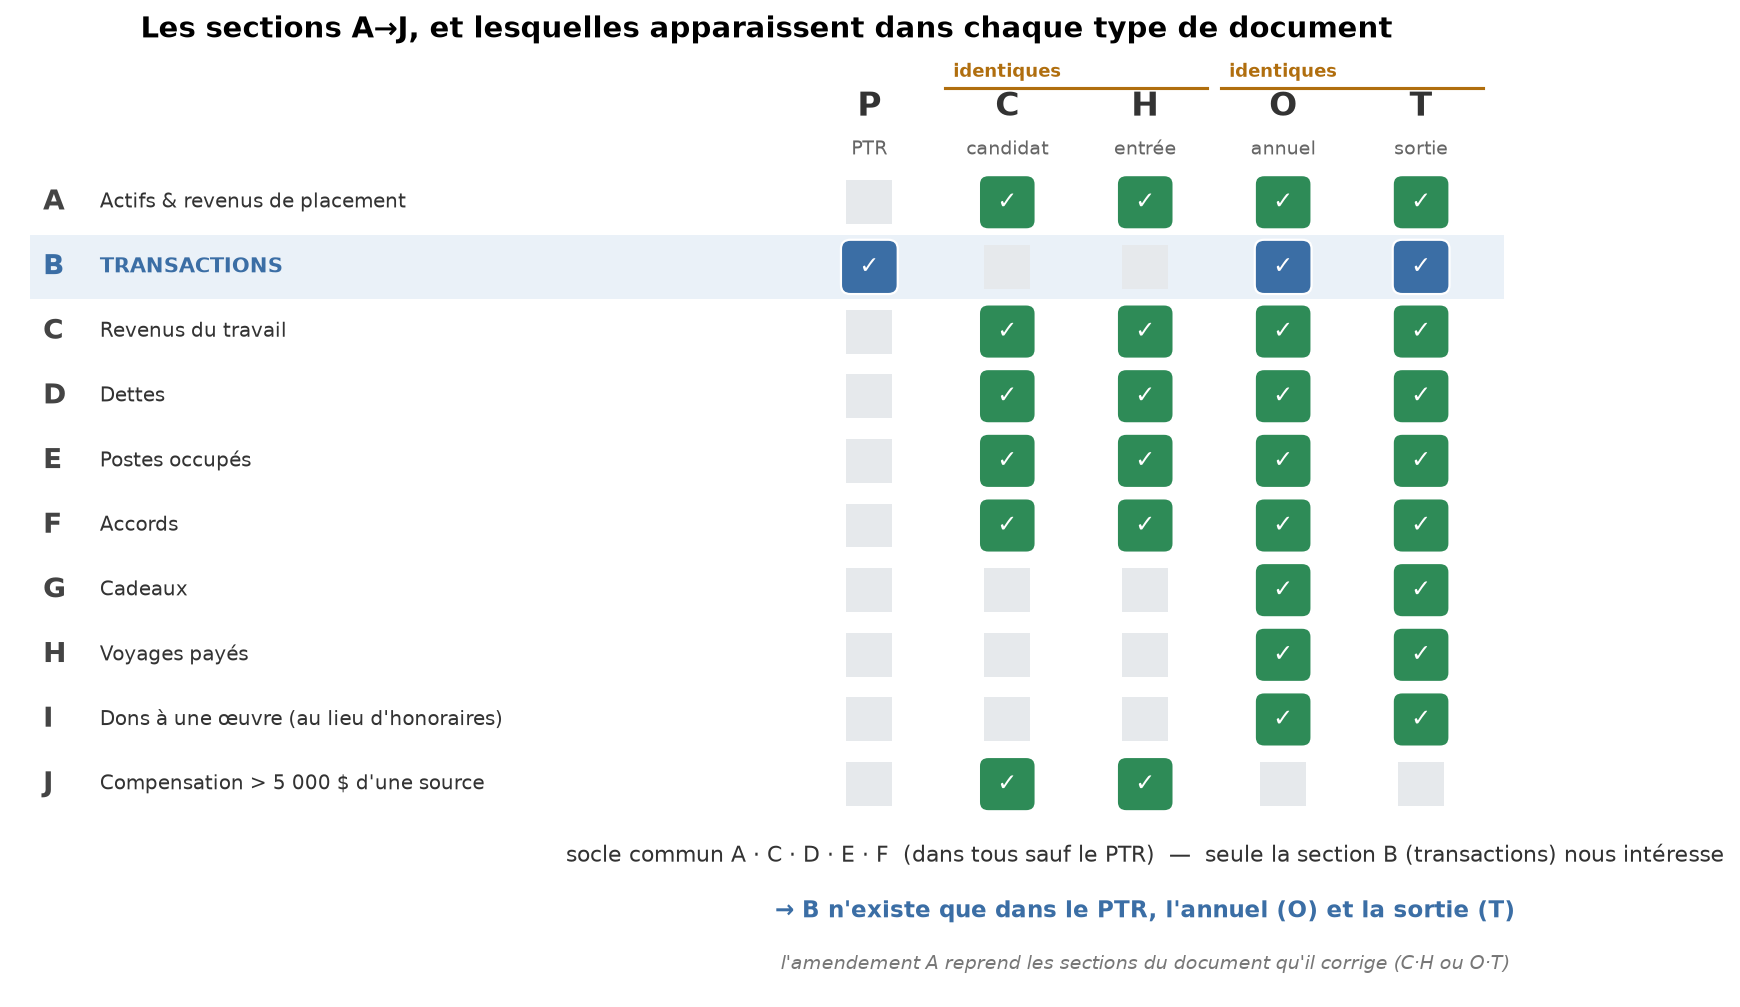
\includegraphics[width=\linewidth,height=0.55\textheight,keepaspectratio]{figs_depots/fig_sections_matrix.png}\\[1mm]
   {\scriptsize\color{black!55} les sections présentes selon le type de dépôt.}
  \end{columns}
\end{frame}

% ── A3 · ce qu'on extrait : A (nouveau) + B ──
\begin{frame}{4 · Extraire --- on ne garde que deux sections : A et B}
  \begin{columns}[T]
  \column{0.5\textwidth}
   \colorbox{okgreen!14}{\parbox[t][3.5cm][t]{\dimexpr\linewidth-8pt}{\vspace{0.6mm}
     {\color{okgreen}\bfseries Schedule A --- patrimoine} \textbf{(le NOUVEAU)}\\[1mm]
     {\footnotesize les \textbf{actifs détenus} (fourchette de valeur, sans date) --- \emph{la photo} du portefeuille. Le PTR ne l'a \textbf{pas} : c'est ce qui rend possible toute la reconstruction (Acte 3).}}}
  \column{0.5\textwidth}
   \colorbox{helec!12}{\parbox[t][3.5cm][t]{\dimexpr\linewidth-8pt}{\vspace{0.6mm}
     {\color{helec}\bfseries Schedule B --- transactions}\\[1mm]
     {\footnotesize les mêmes trades que le PTR, mais \textbf{format différent} (ordre \emph{date · type · montant}) → un \textbf{parseur séparé}.}}}
  \end{columns}
  \vspace{3mm}
  \choixbox{les huit autres sections (\co{C} revenus · \co{D} dettes · \co{E} positions · \co{F} accords · \co{G} cadeaux · \co{H} voyages · \co{I} paiements · \co{J} rémunérations) sont \textbf{ignorées} --- hors sujet portefeuille. Et on ne garde que les lignes \textbf{tickérisées} (le non-coté est compté, pas utilisé).}
\end{frame}

% ── A4 · l'OCR des FD scannés : couverture quasi complète + 2 limites ──
\begin{frame}{4 · Extraire --- l'OCR des FD scannés : quasi complet, limites vérifiées}
  \begin{columns}[T]
  \column{0.5\textwidth}
   \colorbox{helec!12}{\parbox[t][3.9cm][t]{\dimexpr\linewidth-8pt}{\vspace{0.6mm}
     {\color{helec}\bfseries Couverture --- quasi complète}\\[1mm]
     {\footnotesize l'OCR (\co{claude-sonnet-5}, contrat \co{record\_fd}) extrait \textbf{Schedule A + B}. \textbf{2\,842 / 2\,851} FD scannés OCRisés ; les \textbf{9} manquants = reliquats \textbf{2014} (PDF morts). Même les annexes de courtier (jusqu'à \textbf{797 p. / 51\,048 lignes}) sont passées.}}}
  \column{0.5\textwidth}
   \colorbox{dataC!14}{\parbox[t][3.9cm][t]{\dimexpr\linewidth-8pt}{\vspace{0.6mm}
     {\color{dataC}\bfseries Deux limites --- vérifiées}\\[1mm]
     {\footnotesize \textbf{(1)} les \textbf{312 « vides »} sont des \textbf{formulaires blancs} (vérifié en ouvrant les PDF : Schedule A vierge) --- l'OCR a \emph{raison}, pas des ratés. \textbf{(2)} \textbf{5\,185} valeurs mal lues (2,7 \%) --- \textbf{sans effet sur le backtest} (tables FD hors périmètre) ; un fix parseur en récupère \textbf{1\,667}.}}}
  \end{columns}
  \vspace{2.5mm}
  \choixbox{ce qui justifie la dépense : \textbf{29 \%} des documents (scannés) portent \textbf{65 \%} des transactions --- l'OCR payant est \textbf{rentable}. Cache versionné → re-run \textbf{0 \$} (26 JSON rendus en chaîne, réparés au caractère près).}
\end{frame}

% ── A5 · les 18 tables ──
\begin{frame}{5 · Les 18 tables --- le résultat de la collecte}
  \centering\pipestrip{5}\\[2.5mm]
  {\footnotesize
  \begin{tabular}{@{}l p{0.70\linewidth}@{}}
   \toprule
   \textbf{Récupérer / router} & 01 recensement · 02 ledger · 03 inventaire PDF\\
   \textbf{Identifier} & 06 identités\\
   \textbf{Extraire — électronique} & 04 transactions (dédup) · 05 holdings (FD élec)\\
   \textbf{Extraire — OCR scanné} & 07 transactions PTR·OCR · 08 holdings FD·OCR · 09 transactions FD·OCR\\
   \textbf{Comptabilité} & 10 comptabilité du traitement\\
   \textbf{Reconstruire (Acte 3)} & 11 holdings complets · 12 portefeuilles datés · 13·17 recalages · 14 registre · 15 portefeuille d'entrée · 16 flux O/A/T · 18 churn\\
   \bottomrule
  \end{tabular}}\\[2.5mm]
  {\scriptsize\color{black!55} chaque table est \textbf{numérotée, versionnée, re-jouable} --- c'est ce qui empêche la donnée de « partir dans tous les sens ».}
\end{frame}

% ── A6 · la comptabilité boucle ──
\begin{frame}{6 · La boucle --- chaque dépôt a un traitement, la somme boucle}
  \centering\pipestrip{6}\\[3mm]
  \begin{columns}[c]
  \column{0.46\textwidth}
   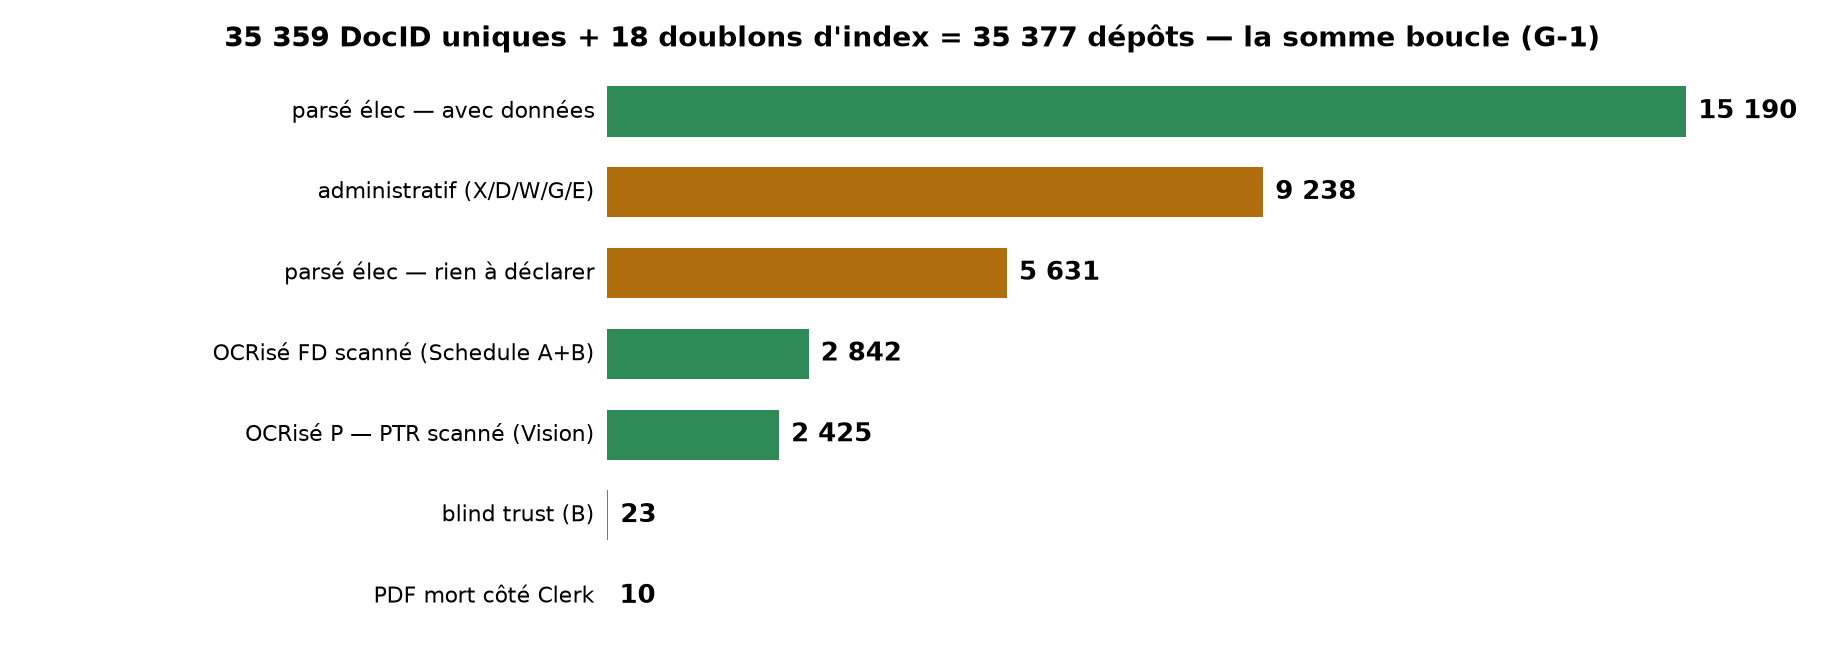
\includegraphics[width=\linewidth,height=0.5\textheight,keepaspectratio]{figs_depots/fig_house_compta.png}
  \column{0.54\textwidth}
   {\footnotesize sur les \textbf{35\,377} recensés :}
   \begin{itemize}\footnotesize
    \item[--] \textbf{20\,457} → \textbf{données extraites} (15\,190 élec + 2\,842 OCR FD + 2\,425 OCR PTR)
    \item[--] \textbf{14\,869} recensés, \textbf{rien à extraire} (administratifs \co{X}/\co{D}/\co{W}/\co{G}/\co{E} + lignes vides)
    \item[--] \textbf{33} hors périmètre (23 blind trust + 10 PDF morts, tracés)
    \item[--] \textbf{18} doublons d'index (retirés)
   \end{itemize}
   \vspace{0.5mm}
   {\footnotesize \textbf{75 contrôles automatiques, 0 rouge} · somme vérifiée par \emph{assert} bloquant.}\\[2mm]
   \repband{chacun des \textbf{27\,110} « autres » dépôts a reçu \textbf{exactement un} traitement --- rien perdu, rien inventé.}
  \end{columns}
\end{frame}

% ════════════════════════════════════════════════════════════
\partdivider{dataC}{ACTE 2}{Les autres dépôts : les chiffres au clair}{un type lu sur douze --- et de quoi parlent tous ces nombres}

% ── A1 · le problème ──
\begin{frame}{Le problème --- on n'avait lu qu'un type de dépôt sur douze}
  \begin{columns}[T]
  \column{0.46\textwidth}
    \colorbox{helec!10}{\parbox[t]{\dimexpr\linewidth-8pt}{\vspace{0.8mm}
      {\Large\textbf{\color{helec}8\,267}}~dépôts \textbf{PTR} lus\\[0.4mm]
      {\scriptsize le seul type exploité jusqu'ici --- « ce que l'élu \emph{fait} »}}}\\[2.2mm]
    \colorbox{dataC!14}{\parbox[t]{\dimexpr\linewidth-8pt}{\vspace{0.8mm}
      {\Large\textbf{\color{dataC}27\,110}}~autres dépôts, \textbf{11 types}\\[0.4mm]
      {\scriptsize jamais lus --- « ce que l'élu \emph{possède} »}}}\\[2.2mm]
    {\footnotesize sur \textbf{35\,377} dépôts recensés (Chambre, 2014--2026).}
  \column{0.52\textwidth}
    {\footnotesize Décomposition du \textbf{patrimoine de sortie} d'un élu :}\\[2mm]
    \begin{tikzpicture}[node distance=1.4mm]
      \node[bande=grisC, text width=6.3cm] (a)
        {\textbf{33,2\%} déjà détenu \textbf{à l'entrée} --- invisible d'un départ de zéro};
      \node[bande=helec, text width=6.3cm, below=of a] (b)
        {\textbf{45,5\%} acheté \textbf{pendant le mandat} --- vu par les PTR};
      \node[bande=dataC, text width=6.3cm, below=of b] (c)
        {\textbf{21,3\%} restait \textbf{à expliquer}};
    \end{tikzpicture}\\[2.5mm]
    \choixbox{les « autres dépôts » sont la matière qui rend visible le \textbf{tiers déjà là} --- c'est tout l'enjeu.}
  \end{columns}
\end{frame}

% ── A2 · le catalogue ──
\begin{frame}{Le catalogue --- douze types de dépôt, trois familles}
  \centering\vspace{0.5mm}
  {\footnotesize
  \begin{tabular}{@{}c l r l@{}}
   \toprule
   \multicolumn{4}{@{}l}{\textbf{\color{dataC}Le signal --- ce que l'élu \emph{fait}}}\\
   \midrule
   \co{P} & Periodic Transaction Report & 8\,267 & les transactions datées (notre backtest)\\
   \midrule
   \multicolumn{4}{@{}l}{\textbf{\color{helec}Les photos du patrimoine --- ce que l'élu \emph{possède}}}\\
   \midrule
   \co{C} & Candidate Report & 10\,129 & patrimoine au moment de la candidature\\
   \co{O} & Annual Report & 4\,626 & bilan annuel\\
   \co{H} & New Filer Report & 395 & photo d'entrée en fonction\\
   \co{T} & Terminated Filer Report & 394 & photo de sortie\\
   \co{A} & Amendment & 2\,305 & correction d'un \co{O}/\co{C}/\co{H}/\co{T}\\
   \midrule
   \multicolumn{4}{@{}l}{\textbf{\color{grisC}Administratif --- ni signal ni patrimoine}}\\
   \midrule
   \co{X}\,\co{D}\,\co{W}\,\co{G}\,\co{E} & extensions, avis de campagne, dérogations & \textasciitilde9\,240 & aucune transaction\\
   \co{B} & Blind Trust & 23 & géré à l'aveugle (cas Phillips)\\
   \bottomrule
  \end{tabular}}\\[2.5mm]
  {\scriptsize\color{black!55} chaque chiffre = un \textbf{nombre de dépôts} (millésime union) · total = 35\,377.}
\end{frame}

% ── A3 · les chiffres, une bonne fois (anti-confusion) ──
\begin{frame}{Les chiffres, une bonne fois --- et les pièges}
  \begin{columns}[T]
  \column{0.5\textwidth}
   {\footnotesize\textbf{\color{dataC}Les dépôts \& les transactions}}\\[1.5mm]
   {\scriptsize
   \begin{tabular}{@{}r l@{}}
    \toprule
    \textbf{35\,377} & dépôts recensés (12 types)\\
    8\,267 & dont \textbf{PTR} (le signal)\\
    27\,110 & dont \textbf{autres} (11 types)\\
    \midrule
    \textbf{161\,076} & \emph{transactions} PTR datées\\
    57\,259 & \emph{transactions} dans les annuels\\
    \bottomrule
   \end{tabular}}
  \column{0.5\textwidth}
   {\footnotesize\textbf{\color{helec}Les gens \& leurs portefeuilles}}\\[1.5mm]
   {\scriptsize
   \begin{tabular}{@{}r l@{}}
    \toprule
    \textbf{900} & membres passés par la Chambre\\
    470 / 463 & entrées / sorties (depuis 2014)\\
    284 & photos d'entrée (252 \co{H} + 32 \co{C})\\
    \midrule
    \textbf{822} & portefeuilles \textbf{reconstruits}\\
    56 & \textbf{vérifiés} de bout en bout\\
    \bottomrule
   \end{tabular}}
  \end{columns}
  \vspace{3.5mm}
  \choixbox{trois pièges : \textbf{(1)} un \emph{dépôt} $\neq$ une \emph{transaction} $\neq$ un \emph{membre} --- on ne les additionne jamais ; \textbf{(2)} « 45 » désigne 45 \emph{membres} (la cohorte testée) \emph{ou} 45 \emph{positions} inexpliquées, selon le contexte ; \textbf{(3)} « 21,3\% » a deux sens (du patrimoine de sortie / des positions inexpliquées).}
\end{frame}

% ── A4 · le cycle de vie ──
\begin{frame}{La vie déclarative d'un élu --- photos contre signal}
  \centering
  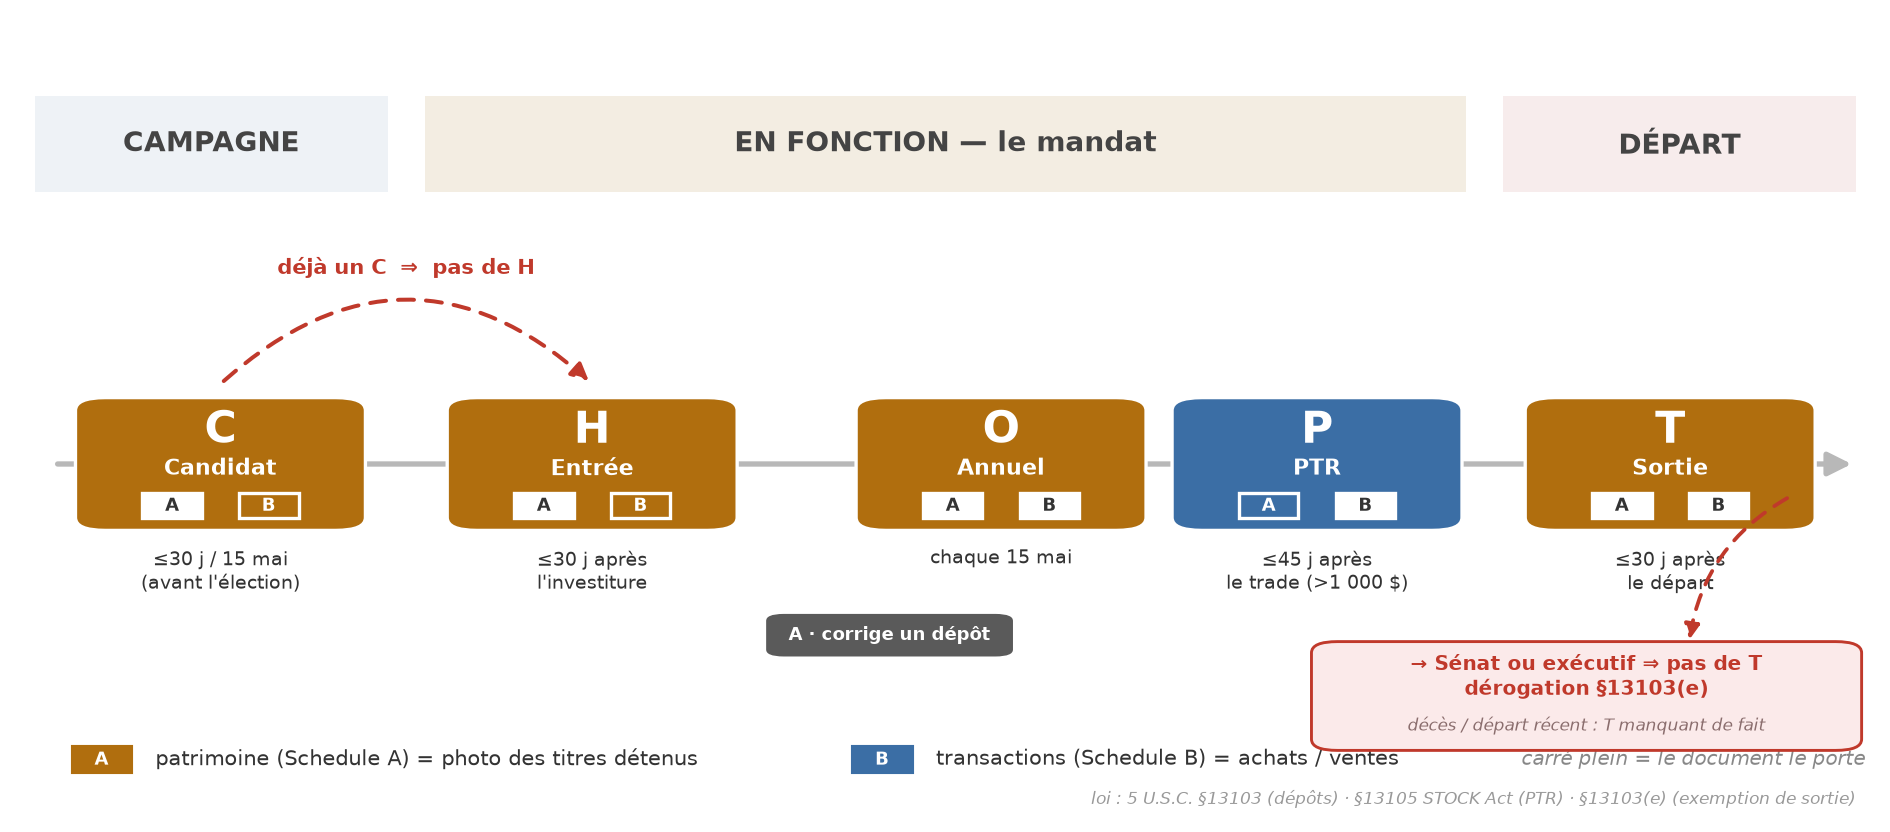
\includegraphics[width=0.92\textwidth,height=0.60\textheight,keepaspectratio]{figs_depots/fig_house_loi_cycle.png}\\[2mm]
  \colorbox{dataC!10}{\parbox{0.92\textwidth}{\centering\footnotesize
    les \textbf{photos} (\co{C}, \co{H}, \co{O}, \co{T}) disent \textbf{ce qu'il possède} (Schedule A) ---
    le \textbf{\co{P}} dit \textbf{ce qu'il fait} (Schedule B). On tradait le \co{P} ; on va se servir des \textbf{photos}.}}
\end{frame}

% ── A5 · couverture entrées/sorties ──
\begin{frame}{La couverture des entrées et des sorties}
  \centering\vspace{2mm}
  {\footnotesize
  \begin{tabular}{@{}p{0.24\linewidth} p{0.64\linewidth}@{}}
   \toprule
   \textbf{470 entrées} au Congrès depuis 2014 & \textbf{82\%} ont déposé un \co{H}, \textbf{16\%} un \co{C} --- \textbf{98\% couvertes} par une photo d'entrée\\
   \midrule
   \textbf{463 sorties} définitives & \textbf{81\%} ont déposé un \co{T} ; les \textbf{86} sans \co{T} = partis au Sénat/exécutif (dispensés), décès\\
   \bottomrule
  \end{tabular}}\\[3mm]
  {\footnotesize la \textbf{photo de départ} : \textbf{252} ancrés par un \co{H} · \textbf{32} par un \co{C} = \textbf{284} portefeuilles d'entrée datés}\\[3mm]
  \choixbox{on distingue \textbf{dépôts} et \textbf{membres} : il y a 395 \emph{dépôts} \co{H} mais 252 \emph{membres} ancrés par un \co{H} (un membre peut en déposer plusieurs ; on ne garde qu'une photo d'entrée).}
\end{frame}

% ── A6 · ce que rate le filtre P ──
\begin{frame}{Ce que rate le filtre PTR --- et pourquoi c'est quand même le bon choix}
  \begin{columns}[T]
  \column{0.5\textwidth}
   {\footnotesize Les Schedule B des annuels (\co{O}/\co{H}/\co{T}/\co{A}) contiennent \textbf{57\,259} transactions :}
   \begin{itemize}\footnotesize
    \item[--] \textbf{79,5\%} \emph{sans ticker} (fonds nommés, immobilier, non coté)
    \item[--] parmi les tickérisées, \textbf{67,1\%} déjà dans nos PTR
    \item[--] reliquat : \textbf{173} actions « annuel-seul » en 13 ans (0,1\%), concentrées 2014--2017
   \end{itemize}
  \column{0.5\textwidth}
   \colorbox{alertred!8}{\parbox[t]{\dimexpr\linewidth-8pt}{\vspace{0.6mm}\footnotesize
     \textbf{\textcolor{alertred}{Le délai tue le signal}}\\[0.6mm]
     divulgation médiane \textbf{406 j} (annuels) contre \textbf{27 j} (PTR) --- impossible à jouer sans regarder l'avenir.}}\\[3mm]
   \repband{le filtre \co{P} reste le bon choix pour le \textbf{signal} ; les annuels ne sont pas un signal --- ils servent de \textbf{vue patrimoine}, ce que l'Acte 2 exploite.}
  \end{columns}
\end{frame}

% ════════════════════════════════════════════════════════════
\partdivider{helec}{ACTE 3}{La population --- qui a quoi}{quatre questions sur les 900 : portefeuille d'entrée, vérifiabilité, annuels --- puis le pont vers le backtest}

% ── B0 · la carte ──
\begin{frame}{La population en une carte --- 900 membres, quatre questions}
  \centering
  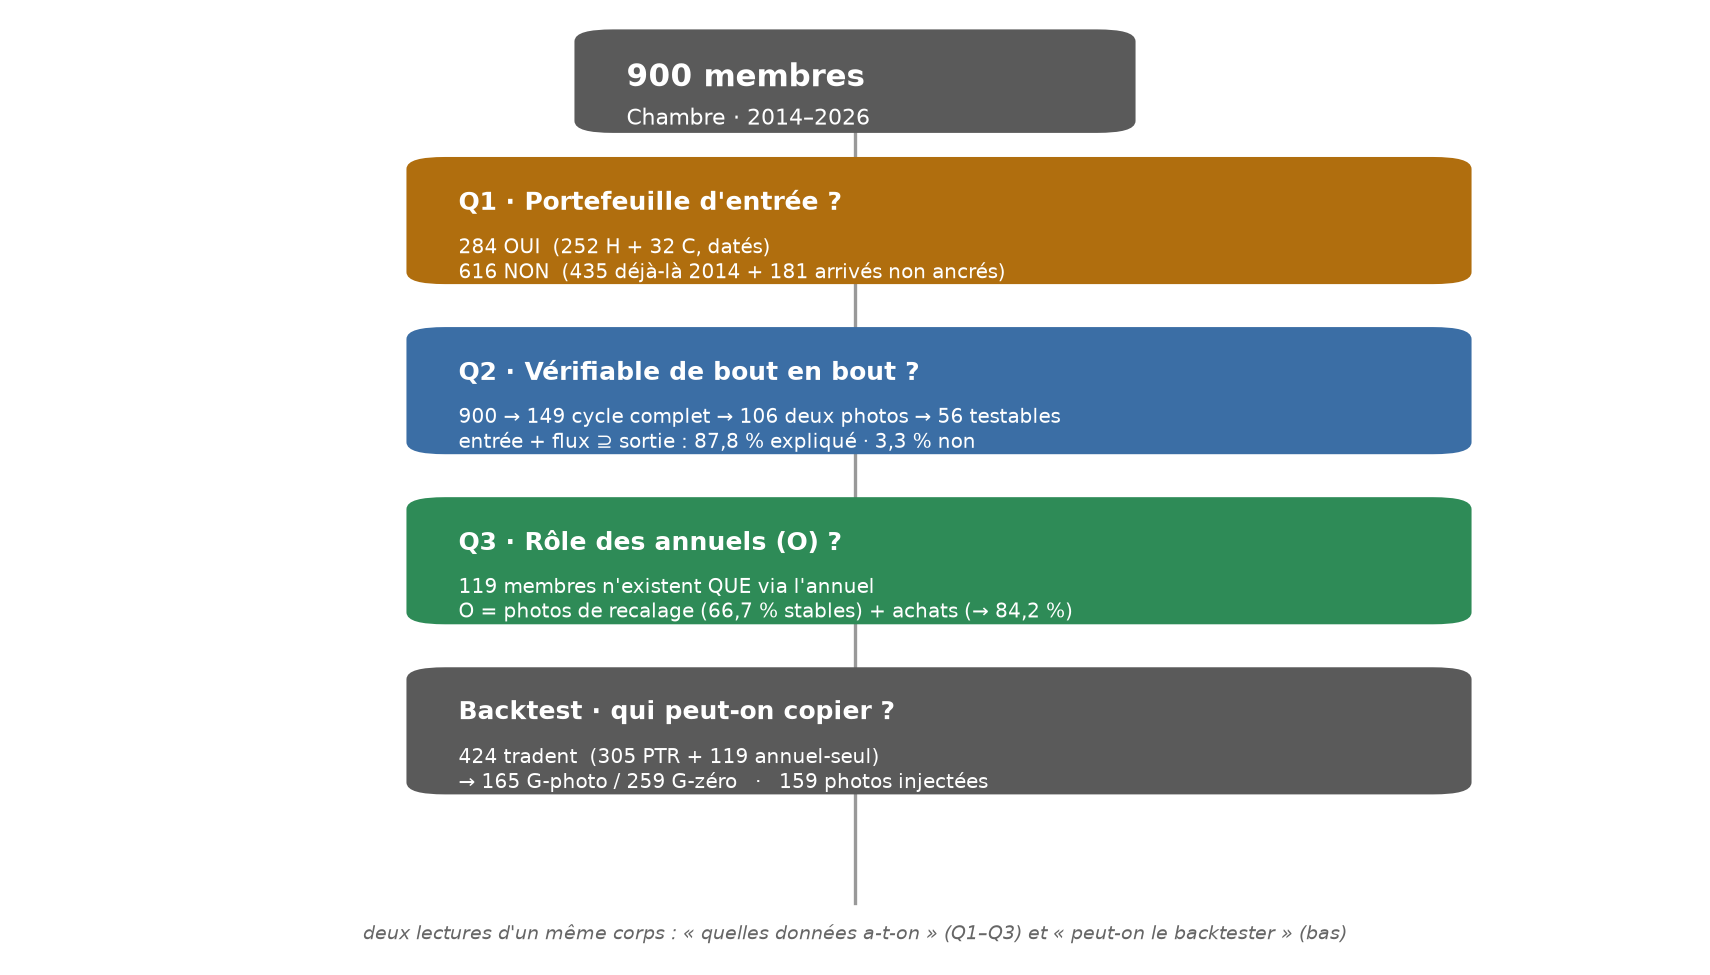
\includegraphics[width=0.97\textwidth,height=0.76\textheight,keepaspectratio]{figs_depots/fig_pop_arbre.png}\\[0.5mm]
  {\scriptsize\color{black!60} deux lentilles sur le même corps : \textbf{quelles données a-t-on} (Q1--Q3) et \textbf{peut-on le backtester} (bas) --- chaque slide qui suit détaille une branche.}
\end{frame}

% ── B1 · Q1 : qui a un portefeuille d'entrée ? ──
\begin{frame}{Q1 · Qui a un portefeuille d'entrée ? --- 284}
  \centering\vspace{1mm}
  \begin{tikzpicture}[node distance=6mm]
    \node[step=grisC, text width=2.5cm, minimum height=1.5cm] (a){\textbf{\large 470}\\{\scriptsize entrées depuis 2014}};
    \node[step=helec, text width=2.5cm, minimum height=1.5cm, right=of a] (b){\textbf{\large 386}\\{\scriptsize ont déposé un \co{H}}};
    \node[step=dataC, text width=2.5cm, minimum height=1.5cm, right=of b] (c){\textbf{\large 252}\\{\scriptsize ancres \co{H} tickérisées}};
    \node[step=okgreen, text width=2.8cm, minimum height=1.5cm, right=of c] (d){\textbf{\large 284}\\{\scriptsize +32 porte \co{C} = portefeuilles d'entrée}};
    \draw[arr](a)--(b); \draw[arr](b)--(c); \draw[arr](c)--(d);
  \end{tikzpicture}\\[3mm]
  {\footnotesize chaque flèche = une perte \emph{mesurée} : \textbf{$-84$} sans \co{H} (75 ont un \co{C}, 9 rien) · \textbf{$-134$} \co{H} \textbf{scannés/OCR} ou patrimoine \textbf{non coté} · \textbf{$+32$} par la \textbf{porte \co{C}} (candidat élec, tickérisé, $\leq$ 1 an avant la prise de poste).}\\[2.5mm]
  \choixbox{« 385 dépôts \co{H} » serait trompeur : il y a 395 \emph{dépôts} bruts, 387 \emph{bioguides}, 386 \emph{entrants} avec \co{H} --- mais seulement \textbf{252} donnent une \emph{photo exploitable}. On compte des \textbf{membres}, pas des dépôts.}
\end{frame}

% ── B2 · Q2 : qui n'en a pas ? ──
\begin{frame}{Q2 · Qui n'a pas de portefeuille d'entrée ? --- 616}
  \vspace{2mm}
  \begin{columns}[T]
  \column{0.5\textwidth}
   \colorbox{grisC!12}{\parbox[t][3.5cm][t]{\dimexpr\linewidth-8pt}{\vspace{0.8mm}
     {\Large\textbf{435}}~structurels\\[1.2mm]
     {\footnotesize déjà en poste en \textbf{2014} : aucune photo d'entrée \emph{possible} dans la fenêtre. Ce n'est pas un trou de collecte.}}}
  \column{0.5\textwidth}
   \colorbox{warnorange!16}{\parbox[t][3.5cm][t]{\dimexpr\linewidth-8pt}{\vspace{0.8mm}
     {\Large\textbf{181}}~arrivés non ancrés\\[1.2mm]
     {\footnotesize entrés après 2014 mais \co{H} \textbf{scanné / sans ticker}, ou aucun dépôt exploitable.}}}
  \end{columns}
  \vspace{3.5mm}
  {\footnotesize\centering \textbf{435 + 181 = 616}\quad et\quad \textbf{284 + 616 = 900}. Pour ces 616, la reconstruction ne peut pas s'ancrer à l'entrée --- elle part d'une photo plus tardive, ou de rien.}
\end{frame}

% ── B3 · le moteur ──
\begin{frame}{Comment on reconstruit --- la mécanique, maths à l'appui}
  \centering\vspace{0.5mm}
  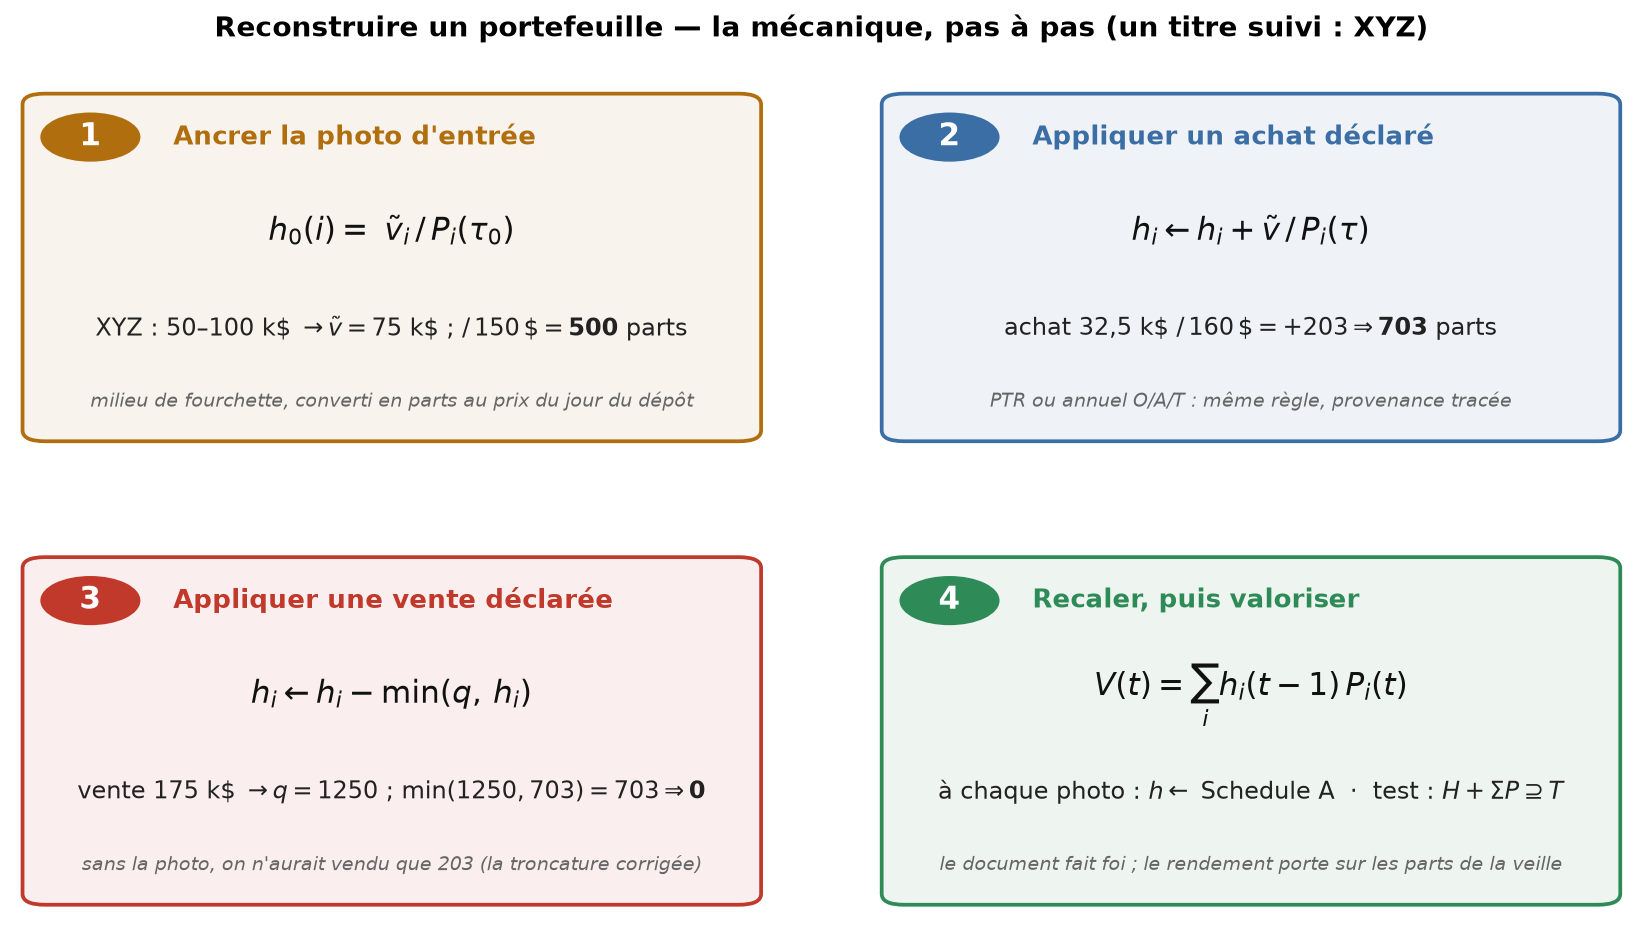
\includegraphics[width=0.93\textwidth,height=0.70\textheight,keepaspectratio]{figs_depots/fig_pop_reconstruction.png}\\[1mm]
  {\scriptsize\color{black!60} en \textbf{parts} (fourchette → milieu → parts au prix du dépôt) · \textbf{66,7\,\%} des positions se confirment d'une photo à la suivante (patrimoine \textbf{stable}, le « churn » = renommage) → \textbf{822} portefeuilles datés.}
\end{frame}

% ── B3bis · sur du vrai : Dean Phillips ──
\begin{frame}{\ldots{}et sur du vrai --- le portefeuille reconstruit de Dean Phillips}
  \centering
  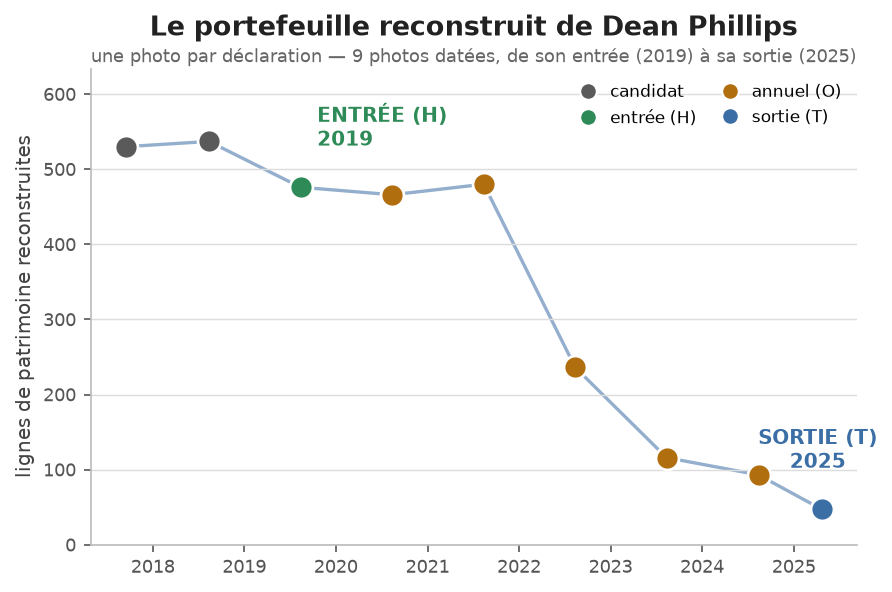
\includegraphics[width=0.82\textwidth,height=0.66\textheight,keepaspectratio]{figs_depots/fig_house_phillips.png}\\[1.5mm]
  {\footnotesize photo d'entrée (\co{H}, 2019) → flux datés → recalage à chaque photo → photo de sortie (\co{T}, 2025) : une \textbf{trajectoire datée} par élu.}
\end{frame}

% ── B4 · Q3 : le test ──
\begin{frame}{Q3 · Qui peut-on vérifier ? --- le test : entrée + achats $\supseteq$ sortie}
  \centering\vspace{1mm}
  {\large $\underbrace{H}_{\text{photo d'entrée}} \;+\; \underbrace{\textstyle\sum P}_{\text{achats déclarés}} \;\supseteq\; \underbrace{T}_{\text{photo de sortie}}$}\\[4mm]
  \begin{tikzpicture}[node distance=7mm]
    \node[bande=grisC, text width=2.5cm] (a){\textbf{900}\\membres};
    \node[bande=helec, text width=2.5cm, right=of a] (b){\textbf{149}\\entrés \emph{puis} sortis};
    \node[bande=helec, text width=2.5cm, right=of b] (c){\textbf{106}\\les 2 photos déposées};
    \node[bande=okgreen, text width=2.5cm, right=of c] (d){\textbf{56}\\actions cotées des 2 côtés};
    \draw[arr](a)--(b); \draw[arr](b)--(c); \draw[arr](c)--(d);
  \end{tikzpicture}\\[4mm]
  {\footnotesize la \textbf{loi} borne l'échantillon : \textbf{439} déjà en poste en 2014 (pas de photo d'entrée), \textbf{437} encore en poste (pas de photo de sortie) ; la moitié des 106 ne détient \textbf{aucune action cotée}.}\\[2mm]
  \choixbox{une \textbf{identité comptable} : si la collecte était trouée, elle casserait ici. Un détecteur de trous, pas une statistique.}
\end{frame}

% ── B5 · Q3 : le résultat ──
\begin{frame}{Q3 · Le résultat --- 78,7 → 84,2 → 87,8\%, et 3,3\% non}
  \begin{columns}[c]
  \column{0.5\textwidth}
   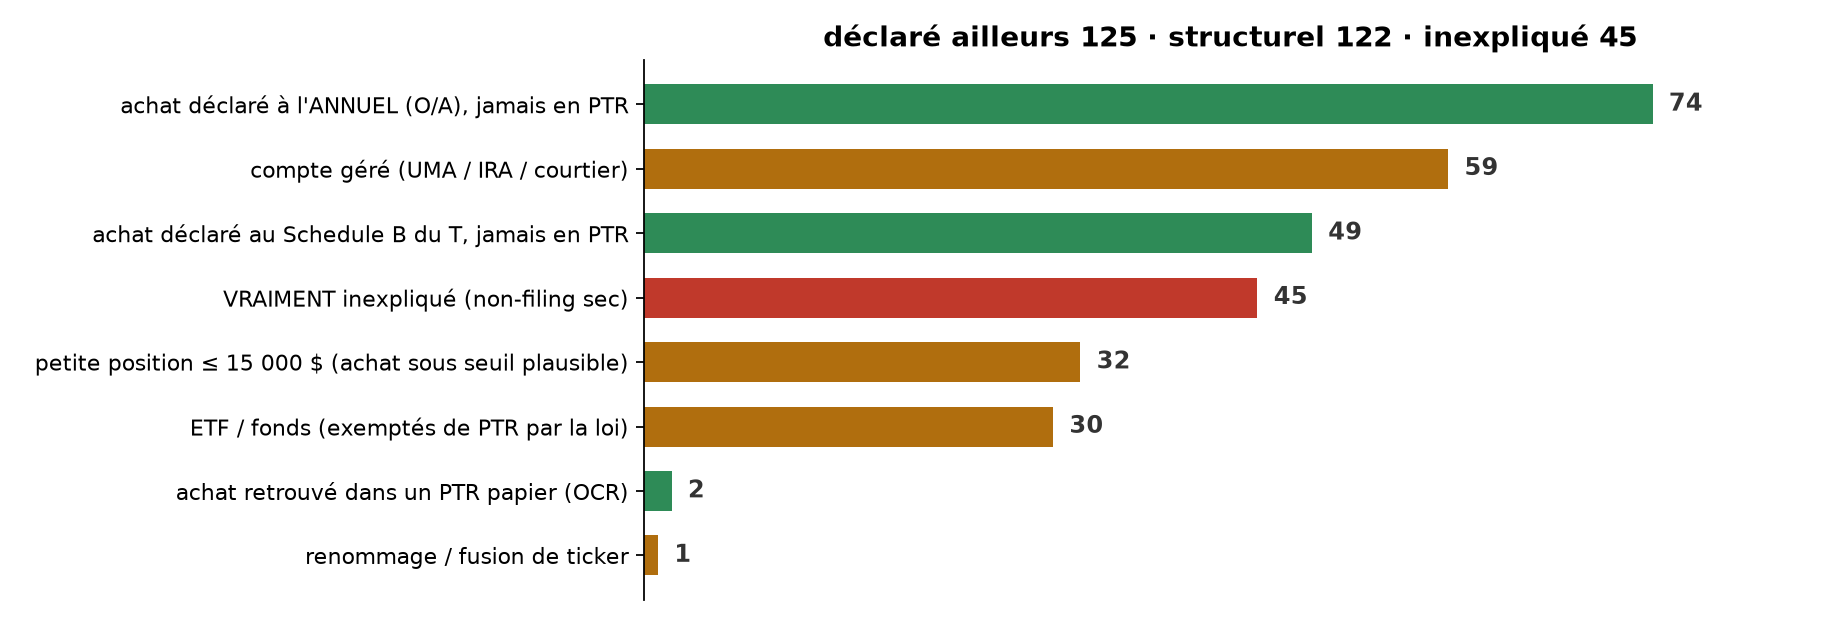
\includegraphics[width=\linewidth,height=0.62\textheight,keepaspectratio]{figs_depots/fig_house_trous.png}
  \column{0.5\textwidth}
   {\footnotesize sur \textbf{1\,371} positions de sortie (cohorte \co{H}∧\co{T} électronique) :}\\[2mm]
   \begin{tikzpicture}[node distance=1.6mm]
     \node[bande=helec, text width=5.8cm] (a){entrée + achats \textbf{PTR} → \textbf{78,7\%}};
     \node[bande=okgreen, text width=5.8cm, below=of a] (b){+ Schedule B des \textbf{annuels} (\co{O}/\co{A}) → \textbf{84,2\%}};
     \node[bande=okgreen, text width=5.8cm, below=of b] (c){+ Schedule B de la \textbf{sortie} (\co{T}) → \textbf{87,8\%}};
     \node[bande=grisC, text width=5.8cm, below=of c] (d){$-122$ structurelles (comptes gérés, ETF, petites lignes)};
     \node[bande=alertred, text width=5.8cm, below=of d] (e){\textbf{45 positions / 14 membres = 3,3\%} inexpliquées};
     \draw[arr](a)--(b); \draw[arr](b)--(c); \draw[arr](c)--(d); \draw[arr](d)--(e);
   \end{tikzpicture}\\[1.5mm]
   \choixbox{chaque écart est \textbf{classé par preuve documentaire}, jamais éliminé statistiquement.}
  \end{columns}
\end{frame}

% ── B6 · Q4 : le rôle des annuels ──
\begin{frame}{Q4 · Le rôle des annuels (\co{O}) --- « sur l'annualisé »}
  \begin{columns}[T]
  \column{0.5\textwidth}
   \colorbox{okgreen!12}{\parbox[t][3.4cm][t]{\dimexpr\linewidth-8pt}{\vspace{0.8mm}\footnotesize
     \textbf{\textcolor{okgreen}{1 · des trades qu'on n'aurait pas}}\\[0.8mm]
     flux annuel net \textbf{26\,115} (\co{O} = 85\,\%) → 14\,970 ajoutés. \textbf{119 membres} n'ont \emph{aucun} trade PTR : leurs seules actions cotées n'existent que \textbf{dans l'annuel}. La population passe de \textbf{305 à 424}.}}
  \column{0.5\textwidth}
   \colorbox{helec!10}{\parbox[t][3.4cm][t]{\dimexpr\linewidth-8pt}{\vspace{0.8mm}\footnotesize
     \textbf{\textcolor{helec}{2 · des points de recalage}}\\[0.8mm]
     les photos \co{O} \textbf{recalent} le portefeuille entre l'entrée et la sortie (\textbf{66,7\,\%} stables), et leur Schedule B fournit le pas \textbf{78,7 → 84,2\,\%} du test.}}
  \end{columns}
  \vspace{2.5mm}
  \choixbox{« vérifier sur l'annualisé » = les trades \co{O}/\co{A}/\co{T} \emph{plus} le patrimoine d'entrée. Le \textbf{backtest} (Acte 3), lui, ne part que de la \textbf{photo d'entrée} --- pas des photos annuelles intermédiaires.}
\end{frame}

% ── B7 · deux compteurs, deux partitions, le croisé ──
\begin{frame}{Deux compteurs, deux partitions --- et le croisement}
  \begin{columns}[c]
  \column{0.42\textwidth}
   {\footnotesize\textbf{Deux questions, jamais confondues :}}\\[1.5mm]
   \colorbox{dataC!12}{\parbox{\dimexpr\linewidth-8pt}{\footnotesize\vspace{0.5mm}
     \textbf{RECONSTRUIRE} → \textbf{822}\\{\scriptsize $\geq$ 2 photos datées}\vspace{0.5mm}}}\\[1.5mm]
   \colorbox{helec!12}{\parbox{\dimexpr\linewidth-8pt}{\footnotesize\vspace{0.5mm}
     \textbf{VÉRIFIER} → \textbf{56}\\{\scriptsize cycle complet, testable}\vspace{0.5mm}}}\\[2.5mm]
   {\scriptsize registre \emph{par force de preuve} : \textbf{56} + \textbf{109} complet + \textbf{715} partiel + \textbf{20} hors = \textbf{900}. 822 et 56 ne s'additionnent pas ; $822 \subset 880$ ($= 900 - 20$).}\\[1.5mm]
   \repband{$\sim$9 reconstruits sur 10 restent sans preuve de bout en bout --- on l'assume. Fil rouge : \textbf{Dean Phillips}, l'un des 56.}
  \column{0.56\textwidth}
   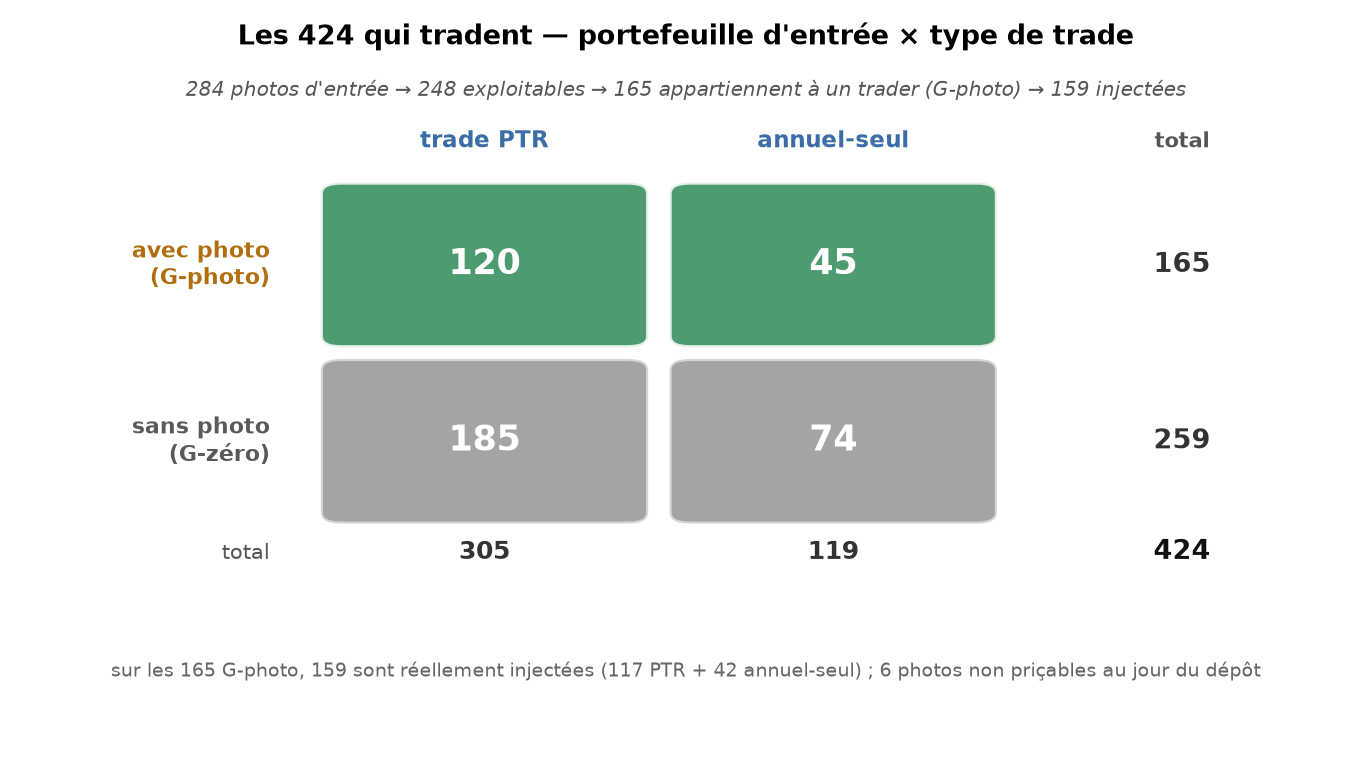
\includegraphics[width=\linewidth,height=0.68\textheight,keepaspectratio]{figs_depots/fig_pop_crosstab.png}
  \end{columns}
\end{frame}

% ════════════════════════════════════════════════════════════
\partdivider{okgreen}{ACTE 4}{Changer la construction du portefeuille}{partir du patrimoine d'entrée au lieu de zéro --- ce que ça change, vraiment}

% ── C1 · l'idée + mécanisme ──
\begin{frame}{L'idée --- partir du patrimoine d'entrée, pas de zéro}
  \begin{columns}[T]
  \column{0.55\textwidth}
   {\footnotesize \textbf{Le mécanisme}, sur un titre suivi (XYZ) :}
   \begin{itemize}\footnotesize
    \item[\textcolor{okgreen}{$\blacktriangleright$}] la \textbf{photo d'entrée} donne \textbf{500 parts} (fourchette convertie au prix du jour du dépôt)
    \item[\textcolor{helec}{$\blacktriangleright$}] un achat déclaré ajoute \textbf{203} parts → \textbf{703}
    \item[\textcolor{alertred}{$\blacktriangleright$}] une vente de \textbf{1\,250} parts : avec la photo on solde $\min(1\,250,\,703)$ ; \textbf{sans} photo le moteur n'aurait vendu que les \textbf{203} achetées --- \textbf{la troncature qu'on corrige}
   \end{itemize}
   \vspace{0.5mm}
   \choixbox{le rendement se calcule sur les parts de la \textbf{veille} : \textbf{un apport n'est jamais une performance} ($r=0$ le jour de l'injection, vérifié numériquement).}
  \column{0.43\textwidth}
   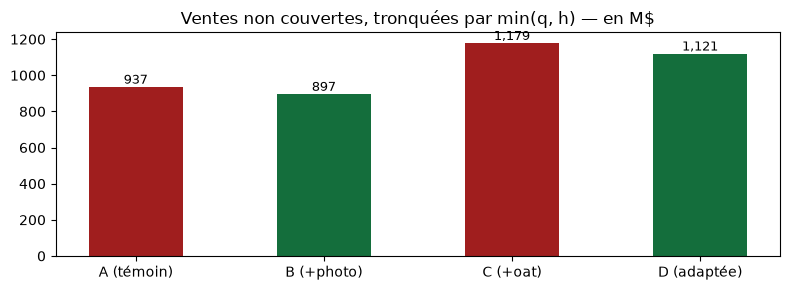
\includegraphics[width=\linewidth]{figs_depots/fig_10_troncature.png}\\[1mm]
   {\scriptsize\color{black!55} ventes non couvertes, tronquées par $\min(q,h)$, en M\$ par run.}
  \end{columns}
\end{frame}

% ── C2 · le dispositif ──
\begin{frame}{Le dispositif --- quatre runs, même moteur, seules les données changent}
  \begin{columns}[T]
  \column{0.52\textwidth}
   \begin{itemize}\footnotesize
    \item[\co{A}] PTR seuls, départ zéro --- \textbf{le témoin}
    \item[\co{B}] \co{A} + photos d'entrée \hfill (\co{B}$-$\co{A} = \textbf{l'effet photo})
    \item[\co{C}] \co{A} + trades \co{O}/\co{A}/\co{T} \hfill (\co{C}$-$\co{A} = \textbf{l'effet \co{O}/\co{A}/\co{T}})
    \item[\co{D}] \co{A} + photos + \co{O}/\co{A}/\co{T} --- \textbf{la stratégie adaptée}
   \end{itemize}
   \vspace{1.5mm}
   {\footnotesize Population : \textbf{900} membres → \textbf{424 tradent} = \textbf{305} vus par les PTR + \textbf{119} \emph{uniquement} via \co{O}/\co{A}/\co{T} → \textbf{165} avec photo exploitable (G\_photo) / \textbf{259} sans (G\_zéro).}
  \column{0.46\textwidth}
   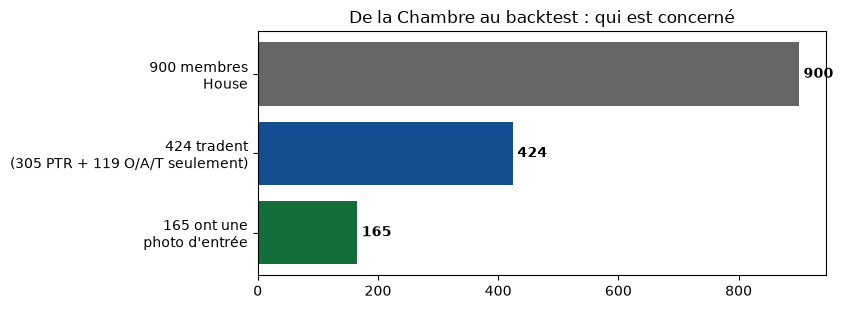
\includegraphics[width=\linewidth]{figs_depots/fig_10_entonnoir.png}
  \end{columns}
\end{frame}

% ── C3 · ce que ça change concrètement ──
\begin{frame}{Ce que ça change concrètement --- qui entre dans le jeu}
  \begin{columns}[T]
  \column{0.45\textwidth}
   {\footnotesize\centering
   \begin{tabular}{@{}l r r r@{}}
    \toprule
    run & membres & photos inj. & tronqué\\
    \midrule
    \co{A} témoin & 226 & 0 & 937 M\$\\
    \co{B} +photo & 257 & 117 & 897 M\$\\
    \co{C} +oat & 362 & 0 & 1\,179 M\$\\
    \textbf{\co{D} adaptée} & \textbf{385} & \textbf{159} & 1\,121 M\$\\
    \bottomrule
   \end{tabular}}\\[2.5mm]
   \begin{itemize}\scriptsize
    \item[--] la photo \textbf{ressuscite 77 vendeurs purs} (31 rendus dès \co{B})
    \item[--] \textbf{42} membres « \co{O}/\co{A}/\co{T}-seuls » enfin servis (\co{D} injecte 159 photos, pas 117)
    \item[--] la \textbf{sélection change à 11/11 coupes} annuelles
   \end{itemize}
  \column{0.53\textwidth}
   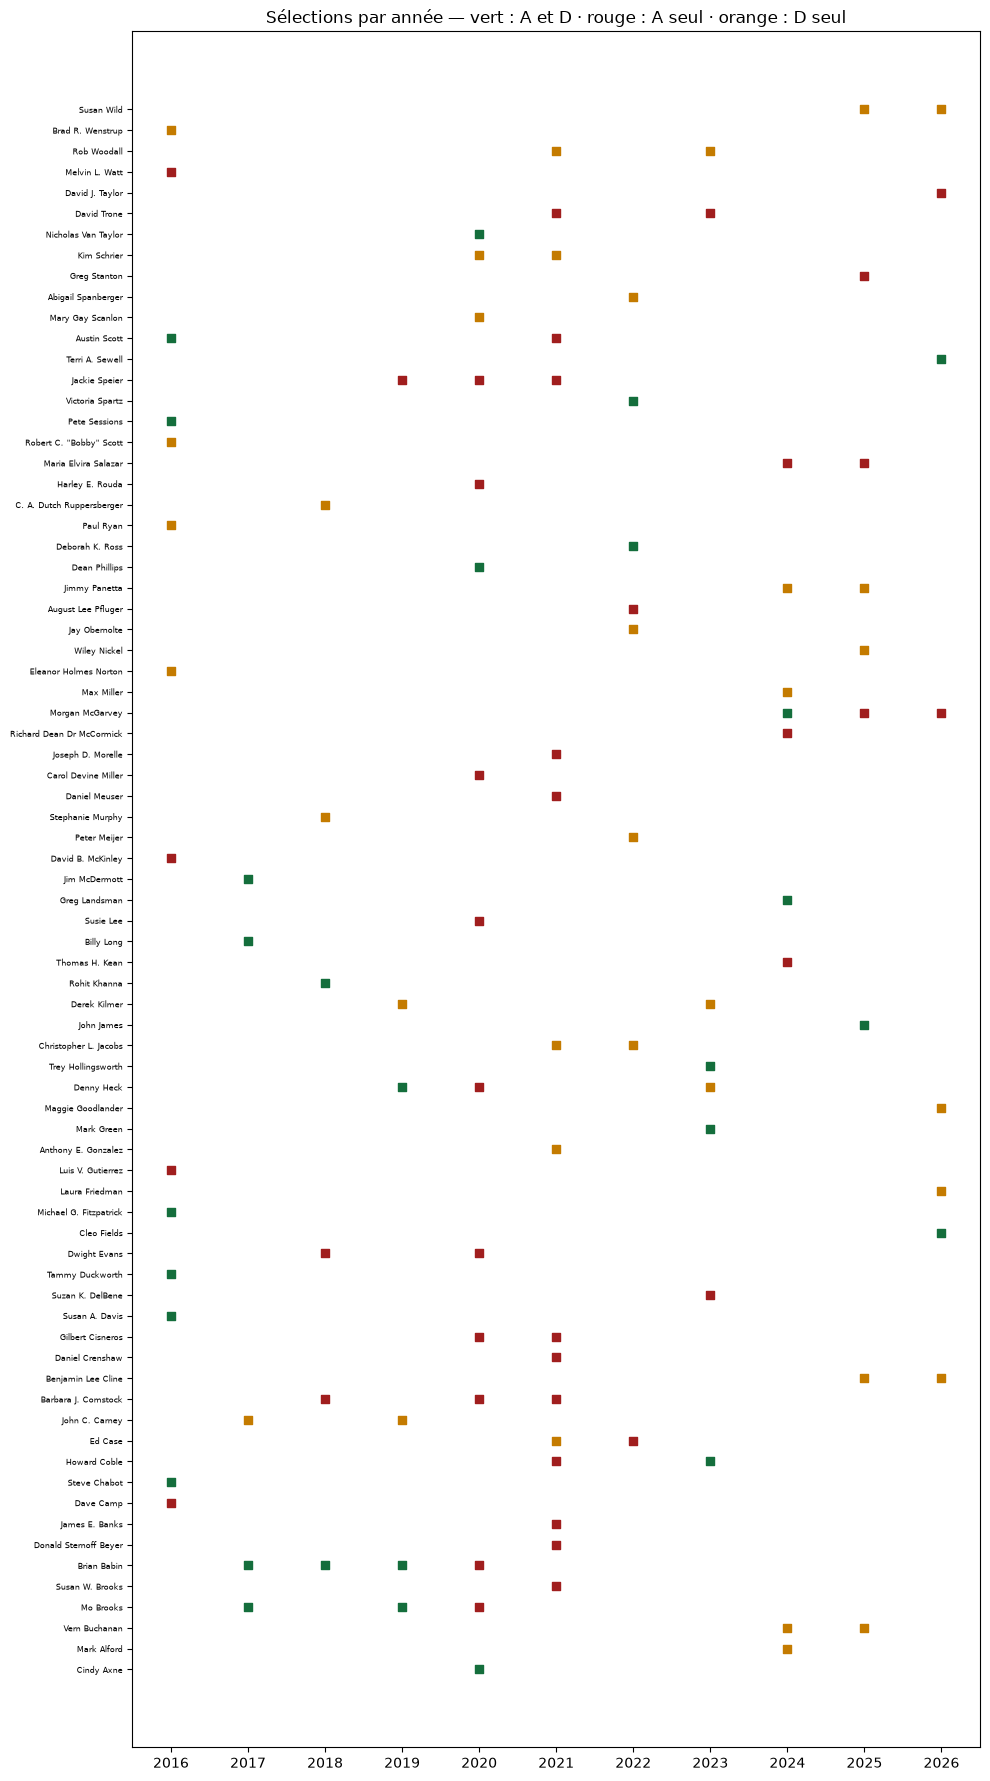
\includegraphics[width=\linewidth,height=0.60\textheight,keepaspectratio]{figs_depots/fig_10_composition.png}\\[1mm]
   {\scriptsize\color{black!55} sélections par année : vert = \co{A} \emph{et} \co{D} · rouge = \co{A} seul · orange = \co{D} seul.}
  \end{columns}
\end{frame}

% ── C4 · le tableau des résultats ──
\begin{frame}{Le tableau --- excès vs SPY, sur 11 années civiles}
  \begin{columns}[T]
  \column{0.55\textwidth}
   {\scriptsize\centering
   \begin{tabular}{@{}l r r l r r@{}}
    \toprule
    run · poids & excès/an & $t$ & gagn. & $\beta$ & $t_{\text{ap}}$\\
    \midrule
    \co{A} · 1/K & +0,9 & 0,37 & 4/11 & 0,99 & 0,28\\
    \co{A} · i-v & $-$0,3 & $-$0,11 & 4/11 & 1,00 & $-$0,27\\
    \textbf{\co{B} · 1/K} & \textbf{+6,6} & \textbf{0,85} & 5/11 & 0,98 & \textbf{1,55}\\
    \co{B} · i-v & +3,1 & 0,60 & 5/11 & 0,93 & 1,33\\
    \co{C} · 1/K & $-$0,0 & $-$0,02 & 4/11 & 0,92 & 0,54\\
    \co{C} · i-v & $-$1,4 & $-$0,81 & 5/11 & 0,83 & 0,48\\
    \textbf{\co{D} · 1/K} & +0,7 & 0,31 & 4/11 & 0,89 & \textbf{0,96}\\
    \co{D} · i-v & $-$0,6 & $-$0,31 & 4/11 & 0,82 & 0,87\\
    \bottomrule
   \end{tabular}}\\[2mm]
   {\scriptsize\color{black!60} seuil de significativité : $t_{10}\approx 1{,}81$ · l'inverse-vol (i-v) perd sur toutes les lignes.}
  \column{0.44\textwidth}
   
\includegraphics[width=\linewidth]{figs_depots/fig_10_nav.png}\\[1mm]
   {\scriptsize\color{black!55} NAV témoin (\co{A}) vs adaptée (\co{D}) vs SPY, poids 1/K.}
  \end{columns}
\end{frame}

% ── C5 · le mélange surveillé ──
\begin{frame}{Le mélange des deux groupes --- surveillé, pas ignoré}
  \begin{columns}[c]
  \column{0.5\textwidth}
   {\footnotesize \textbf{Le risque :} le Sharpe de G\_photo (portefeuille complet, NAV lisse) et de G\_zéro (base étroite, bruitée) ne se mesurent pas pareil --- le top-$K$ pourrait préférer un groupe pour des raisons de \emph{mesure}, pas de talent.}\\[2mm]
   \begin{itemize}\scriptsize
    \item[\textbf{S1}] le top-$K$ sur-représente G\_photo certaines années (2020 : \textbf{80\%} vs 30\% des éligibles) --- et 0\% d'autres années : le mélange pèse réellement
    \item[\textbf{S2}] jouée \emph{dans chaque groupe séparément}, aucune strate ne contredit le verdict mixte
   \end{itemize}
   \vspace{0.5mm}
   \choixbox{honnêteté : un $t_{\text{ap}}$ de 1,76 vu avant réparation était en partie un \textbf{artefact d'étiquetage} (40 membres à photo classés « zéro ») --- corrigé.}
  \column{0.5\textwidth}
   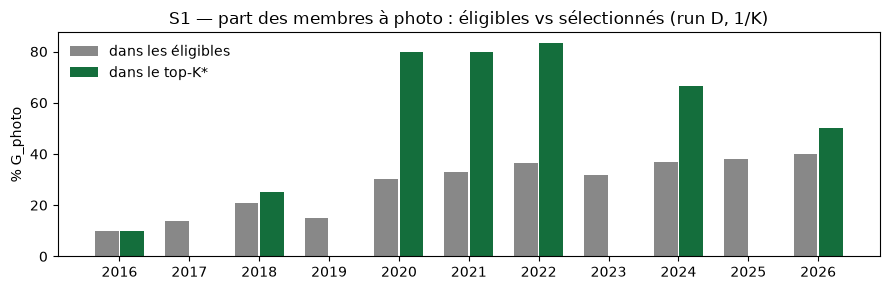
\includegraphics[width=\linewidth,height=0.62\textheight,keepaspectratio]{figs_depots/fig_10_s1.png}
  \end{columns}
\end{frame}

% ── C6 · le verdict ──
\begin{frame}{Le verdict --- plus propre, mais pas d'alpha}
  \vspace{1mm}
  \begin{columns}[T]
  \column{0.5\textwidth}
   \colorbox{alertred!8}{\parbox[t][3.1cm][t]{\dimexpr\linewidth-8pt}{\vspace{0.8mm}
     {\color{alertred}\bfseries Pas d'alpha démontrable}\\[1.5mm]
     {\footnotesize aucune configuration ne franchit le seuil : \textbf{max $t=0{,}85$}, max $t_{\text{ap}}=1{,}59$ en strate. Robuste au poids, à la strate, au mélange \emph{et} au périmètre.}}}
  \column{0.5\textwidth}
   \colorbox{okgreen!12}{\parbox[t][3.1cm][t]{\dimexpr\linewidth-8pt}{\vspace{0.8mm}
     {\color{okgreen}\bfseries Mais un backtest plus propre}\\[1.5mm]
     {\footnotesize l'adaptée resserre le $\beta$ (\textbf{0,99 → 0,89}) et remonte le $t_{\text{ap}}$ (+0,28 → +0,96) ; l'\textbf{effet photo} (\co{B}) est la meilleure ligne, \textbf{+6,6\%/an}.}}}
  \end{columns}
  \vspace{2.5mm}
  {\scriptsize\color{black!60}\textbf{Caveats assumés :} \co{O}/\co{A}/\co{T} datés à la transaction mais divulgués \textasciitilde374 j après · double comptage possible avant le dépôt · non-coté hors périmètre · \co{prices\_v2} jamais modifié.}\\[2.5mm]
  \repband{partir du patrimoine d'entrée est un gain de \textbf{propreté et de robustesse} (moins de bruit de mesure, $\beta$ vers 1) --- pas un alpha nouveau.}
\end{frame}

% ══════════════════════════ CLÔTURE ══════════════════════════
\begin{frame}{Ce qu'on retient}
  \vspace{2mm}
  \begin{itemize}\small
   \item[\textcolor{dataC}{\textbf{1}}] on n'avait lu qu'un dépôt sur douze ; les \textbf{27\,110 autres} rendent visible le \textbf{tiers} du patrimoine « déjà là, jamais tradé ».
   \item[\textcolor{helec}{\textbf{2}}] on \textbf{reconstruit 822} portefeuilles datés et on en \textbf{vérifie 56} de bout en bout : \textbf{87,8\%} des positions de sortie s'expliquent, \textbf{3,3\%} restent, classées par preuve.
   \item[\textcolor{okgreen}{\textbf{3}}] initialiser le backtest au \textbf{patrimoine d'entrée} corrige les ventes tronquées et change les élus copiés --- le résultat est plus \textbf{propre} ($\beta \to$ 1), \textbf{pas} un alpha nouveau.
  \end{itemize}
  \vspace{4mm}
  {\footnotesize\color{black!55} Chambre uniquement · chiffres issus des notebooks V1-House \& 10 · millésime union (35\,377 dépôts).}
  \label{endmain}
\end{frame}

\end{document}
